\usetikzlibrary {automata,positioning}
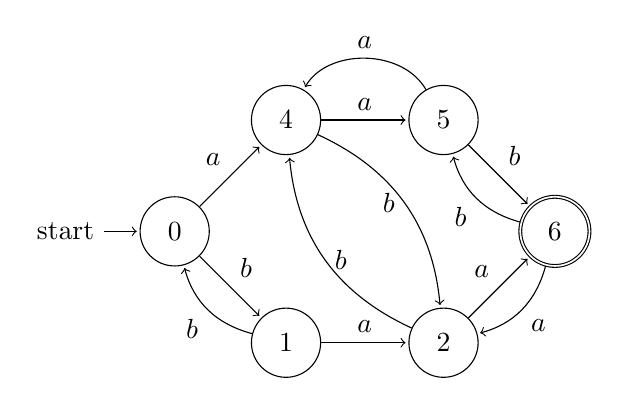
\begin{tikzpicture}[shorten >=1pt,node distance=2cm,on grid,auto]
	\node[initial,state] (0) {0};
	\node[state,below right of=0] (1) {1};
	\node[state,right of=1] (2) {2};
	\node[accepting,state,above right of=2] (6) {6};
	\node[state,above right of=0] (4) {4};
	\node[state,right of=4] (5) {5};
	\path (0) edge [->] node {$b$} (1)
		(1) edge[->] node {$a$} (2)
		(2) edge[->] node {$a$} (6)
		(0) edge[->] node {$a$} (4)
		(4) edge[->] node {$a$} (5)
		(5) edge[->] node {$b$} (6)
		(5) edge[->,out=120,in=60] node[above]  {$a$} (4)
		(6) edge[->,bend left] node {$b$} (5)
		(1) edge[->,bend left] node {$b$} (0)
		(6) edge[->,bend left] node {$a$} (2)
		(4) edge[->,bend left] node[left] {$b$} (2)
		(2) edge[->,bend left] node[right] {$b$} (4);
\end{tikzpicture}
